\part{Ejercicio 1}
\section{Enunciado}
Un torneo de Tenis de eliminaci'on simple consiste en varios partidos donde el perdedor de
cada partido es eliminado del torneo y no vuelve a jugar un partido en ese torneo. El fixture
del torneo se arma al comienzo del mismo tomando dos jugadores a'un no eliminados para
cada partido, hasta que quede s'olo un jugador no eliminado, que resulta ser el ganador.

Con este esquema de fixture no s'olo la destreza o el entrenamiento entran en juego para
decidir el ganador sino que la suerte tiene un papel importante.

Despu'es de observar el entrenamiento de los participantes hay ciertos partidos de los
cuales se puede saber con certeza su resultado, es decir, para ciertos jugadores a,b, se
puede asegurar que a le gana a b.

Diremos que el torneo puede ser arreglado para que gane x si existe un fixture de elimi
naci'on simple donde se puede asegurar que gane x.
Encontrar todos los participantes x para los cuales el torneo puede ser arreglado para gane
x.

Modelar este problema utilizando grafos. Justificar el modelo.

El mejor algoritmo que conocemos es de O(n + m).

\section{Desarrollo}
\subsection{Sobre el modelo}
Para resolver el problema, planteamos un d�grafo donde cada nodo es un jugador y a$\leadsto$b si  a le gana a b. 

Lo primero que observamos es que la relaci�n de ganar, por como esta planteada, es transitiva. Decimos que es transitiva en el sentido de que si a$\leadsto$b y b$\leadsto$c, se puede hacer que a le gane a c, haciendo que b le gane a c y luego a le gane a b. Es decir, si bien a$\leadsto$c, se puede organizar los partidos para que a pueda ganar.

Entonces seg�n este modelo, un jugador, jugador A, puede ganar si para cada uno de los otros jugadores, jugador B, existe un 
camino dirigido que comunica a A con B. Luego si usamos esto, podemos obtener una primera forma de resolver el problema: Para 
cada nodo, tratamos de recorrer todo el grafo. Si lo logramos, se puede armar un torneo para que gane. Como esto se hace para 
cada nodo, el orden queda $O(n*m)$. 

Por otro lado, podemos ver que para que exista un ganador es necesario que si participan n jugadores, la cantidad de partidos arrelgados sea como m�nimo n - 1, ya que con menos partidos, necesariamente quedan jugadores sin un partido arreglado. De modo que obtenemos una caracteristica que permite resolver un tipo de instancia particular muy facilmente.

Buscamos entonces alguna forma de mejorar el orden. Una primera alternativa era guardar 
alguna informaci�n en cada recorrida, para no repetir c�lculos, pero los ciclos nos imped�an lograr alguna soluci�n. Tuvimos  entonces que buscar alguna otra forma.

\subsection{Resolucion en grafos aciclicos}
Si el grafo que se obtiene no presenta ciclos, se puede ver que existe un ganador si y solo si existe un �nico nodo tal que su 
grado de entrada es 0. Por ejemplo, el grafo de la figura ~\ref{fig:conGanador}:

\begin{figure}[H]
\centering
\includegraphics[scale=0.5]{./figuras/conGanador.png}
\caption{Ejemplo con un solo nodo con grado de entrada nulo}
 \label{fig:conGanador}
\end{figure}
En este caso, solo puede haber un ganador, el jugador 1.

Si existen varios, no se podr�n eliminar nunca, ya que no hay quien les gane con seguridad. Por ejemplo, lo grafos de la figura ~\ref{fig:sinGanador}:

\begin{figure}[H]
    \begin{minipage}{.5\linewidth}
    \centering
     \includegraphics[scale=0.5]{./figuras/sinGanador1.png}
    \end{minipage}
    \begin{minipage}{.5\linewidth}
    \centering
      \includegraphics[scale=0.5]{./figuras/sinGanador2.png}
    \end{minipage}
 \caption{Ejemplos con mas de un nodo con grado de entrada nulo}
 \label{fig:sinGanador}
\end{figure}
\afterpage{\clearpage}
En el primer caso, el 5 y el 1 no se pueden eliminar. An�logamente, en el segundo caso, 1 y 6 no se pueden eliminar en ning�n momento.
Por otro lado, no puede ocurrir que no halla ningun nodo con grado de entrada 0, porque si eso ocurre existe un ciclo. (Ver 
demostraci�n 1).

Entonces si no hay ciclos, podemos resolver f�cilmente el problema: Si representamos el grafo con listas de adyacencia (tanto 
de entrada, como de salida), podemos mirar cada nodo, viendo si hay solo uno con grado de entrada 0. Si es as�, ese gana. Si 
encontramos varios, no existe ganador. Esto tiene como costo O(n), ya que recorremos todos los nodos, y preguntamos cuanto mide 
su lista de adyacencia de salida (costo constante).

Ahora bien, no se puede afirmar que el grafo que recibimos no presente ciclos. Es decir hay instancias validas que poseen 
ciclos, por ejemplo la figura ~\ref{fig:conCiclo}:

\begin{figure}[H]
\centering
\includegraphics[scale=0.5]{./figuras/conCiclo.png}
\caption{Ejemplo sin ningun nodo con grado de entrada 0}
 \label{fig:conCiclo}
\end{figure} 
En este caso, el torneo puede arreglarse tanto para 1, como para 2,4 o 5. Debemos entonces buscar alguna manera de salvar esta dificultad.

\subsection{El papel de las componentes fuertemente conexas}
Si tenemos ciclos, no vale la propiedad antes enunciada sobre los grados de entrada.

Analizamos entonces que ocurre si el grafo presenta un ciclo. Como la relaci�n a$\leadsto$b es transitiva (en el sentido que 
comentamos antes), todos los elementos que pertenecen a un ciclo, se ganan entre si. Por otro lado, si tomamos un elemento que 
no este en el ciclo (a) y que le gane a alguien del mismo (b), podemos ver que les puede ganar a todos: primero hacemos que b 
le gane a todos los del ciclo, y luego hacemos que a le gane a b. An�logamente se puede ver que si alguien del ciclo, le gana a 
alguien que no esta en el; cualquier otro del ciclo le puede ganar.

Esto nos hace pensar que podemos considerar al cada ciclo como una unidad, como un jugador �nico, que les gana a todos 
aquellos que son derrotados por alg�n individuo del ciclo y que pierde contra todos aquellos que le ganan a alguien del ciclo.

\begin{figure}[H]
    \begin{minipage}{.5\linewidth}
    \centering
     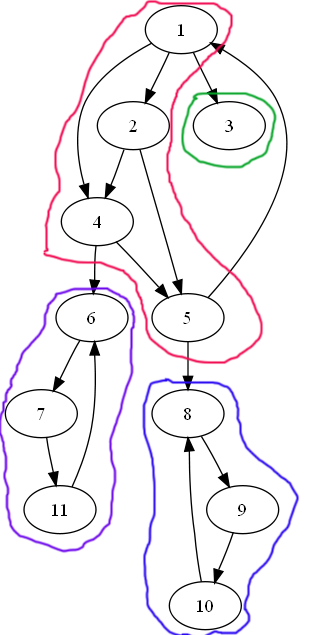
\includegraphics[scale=0.5]{./figuras/componentesConexas.png}
    \end{minipage}
    \begin{minipage}{.5\linewidth}
    \centering
      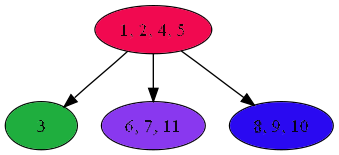
\includegraphics[scale=0.7]{./figuras/reducido.png}
    \end{minipage}
 \caption{Ejemplo de reducci'on de un grafo}
 \label{fig:reduccion}
\end{figure}
%\afterpage{\clearpage}

Estos ciclos que buscamos no son mas que las componentes fuertemente conexas del grafo. Si reducimos al grafo de modo de que 
colapsamos a los nodos que pertenecen a una componente fuertemente conexa a un �nico nodo (como muestra la figura: ~\ref{fig:reduccion}), actualizando la informaci�n de los 
partidos arreglados, lo que obtenemos es un nuevo grafo que cumple ser libre de ciclos (ver demostracion 2).

Entonces una vez que tenemos un grafo libre de ciclos, podemos aplicar la propiedad que enunciamos antes, y resolver el problema en $O(n)$.


\subsection{Obtenci�n de las componentes fuertemente conexas}
Para poder eliminar los ciclos, buscamos las componentes fuertemente conexas. Para hacerlo utilizamos el algoritmo de Kosaraju. 
El mismo logra encontrarlas en O(n+m). El algoritmo es b�sicamente DFS.

Funciona de la siguiente manera:
\begin{itemize}
\item Primero realiza un DFS numerando los nodos seg�n el orden de finalizaci�n de las llamadas recursivas. (se repite hasta numerar todos los nodos).

\item Luego se arma el grafo $g'$ que contiene los mismos nodos que g pero a$\leadsto$b en $g'$ si y solo si b$\leadsto$a en g. g' tiene como caracteristica que posee las mismas componentes conexas que g. Ademas si existe un camino entre dos vertices u y v en g, vale que existe un camino entre u y v en g' si y solo si estan en la misma componente fuertemente conexa.

\item Una vez armado $g'$, se realiza un DFS en 'el, partiendo del nodo con mayor numeraci'on. Al terminar se obtiene una componente fuertemente conexa. 

\item El proceso se repite para todos los nodos no visitados, siempre en orden decreciente de numeraci'on.

\end{itemize}
Como lo que hace el algoritmo es DFS dos veces, tiene orden O(n+m)

Por ejemplo, apliquemos el algoritmo al grafo de la figura ~\ref{fig:kosaraju1}:

\begin{figure}[H]
\centering
\subfigure[Comenzamos con el grafo original]{
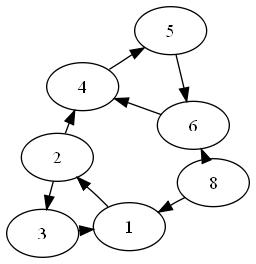
\includegraphics[scale=0.6]{./figuras/kosaraju1.png} }\hspace{1in} 
\subfigure[Realizamos DFS partindo desde el 1 y numeramos los nodos segun el orden de la llamada recursiva]{
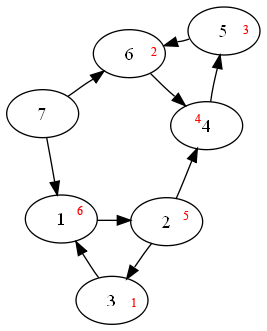
\includegraphics[scale=0.6]{./figuras/kosaraju2.png}}
\subfigure[Como el 8 quedo sin marcar, realizamos una segunda DFS partiendo desde el]{
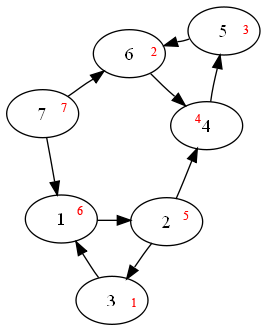
\includegraphics[scale=0.6]{./figuras/kosaraju3.png}}\hspace{1in} 
\subfigure[Una vez que marcamos todos los nodos, invertimos el grafo]{
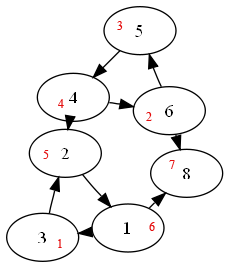
\includegraphics[scale=0.6]{./figuras/kosaraju4.png}} 
\subfigure[Como el 8 es el elemento de mayor numeraci'on comenzamos por �l. Hacemos DFS, y todos los nodos que tocamos, son una componente fuertemente conexa]{
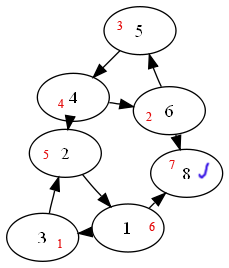
\includegraphics[scale=0.6]{./figuras/kosaraju5.png} }\hspace{1in} 
\subfigure[Ahora seguimos con el 1, el de mayor numeraci'on sin visitar. Luego de hacer DFS tenemos otra componente fuertemente conexa de G. Como no quedan mas nodos por visitar, terminamos]{
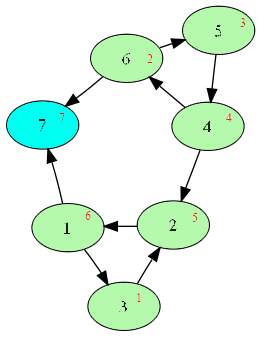
\includegraphics[scale=0.6]{./figuras/kosaraju6.png}}
\caption{Algoritmo de Kosaraju}
\label{fig:kosaraju1}
\end{figure}

\subsection{Armado del grafo reducido y resoluci�n del problema}
Una vez que ya tenemos las componentes fuertemente conexas, armar el grafo reducido es simple. 
\begin{itemize}
\item Primero guardamos en que componente quedo cada jugador

\item Luego tomamos las relaciones entre los jugadores, y las traducimos al nuevo grafo: las 
releciones dentro de la misma componente se descartan, y dos componentes estan relacionadas si existe un jugador en cada una, 
tal que esten relacionados.Es de notar que es necesario filtrar las relaciones intracomponente para no obtener un 
pseudografo que no nos permite usar la propiedad de los grafos sin ciclos, pues un nodo queda relacionado con si mismo, por lo 
que tiene grado de entrada mayor  a 0. Tambien es de notar que no podemos obtener un multigrafo, ya que el grafo es libre de 
ciclos: si vale que a$\leadsto$b y b$\leadsto$a, a y b deberian ser una unica componente fuertemente conexa.

\item Con esta informaci�n podemos armar el nuevo grafo.

\item Contamos cuantos elementos tienen grado de llegada 0, si solo hay uno ese gano. Entonces ganan todos los elementos de la componente. Como podrian no estar en orden, las ordenamos mediante bucket sort en $O(n)$

\end{itemize}

\subsection{Demostraciones auxiliares}
\newtheorem{teorema 1}{Teorema}
\begin{teorema 1}
\normalsize
Sea g=(V,X) tal que $\forall$ v $\in$ V, $d_{in}(v)$ $>$ 0 $\Leftarrow$ existe un ciclo en g
\end{teorema 1}

\renewcommand*{\proofname}{Demostraci�n}

\begin{proof}
\normalsize
Sea g=(V,X) tal que  $\forall$ v $\in$ V, d(v) $>$ 0, consideremos el camino maximo de g, $v_1,v_2,...v_i,...,v_n$
\begin{figure}[H]
\centering
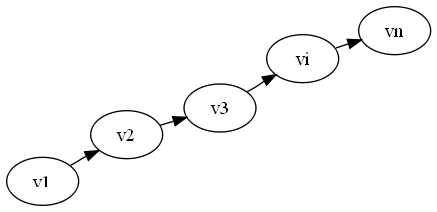
\includegraphics[scale=0.5]{./figuras/demostracion.png}
\end{figure} 
Pero como f $d_{in}(v)$ $>$ 0, existe $v_k$ tal que $v_k$ $\leadsto$ $v_1$. Si $v_k$ pertenece al camino, tenemos un ciclo, que era lo que quer'iamos demostrar.
Supongamos que no pertenece al camino. Entonces tengo un camino nuevo, que va de $v_k$ a $v_n$, que tiene mayor longitud que
el camino de $v_1$ a $v_n$, absurdo, puesto que $v_1,v_2,...v_i,...,v_n$ era el camino m�ximo.
\end{proof}
\vspace{0.2in}
\begin{teorema 1}
\normalsize
Sea g un grafo reducido, es decir que cada nodo es una componente fuertemente conexa, entonces no existen circuitos en g
\end{teorema 1}
\begin{proof}
\normalsize
Supongamos que existe un circuito en g. Sean $a_1$,$a_2$,..., $a_i$,..., $a_n$ nodos, tal que el circuito pasa por ellos. Como tengo un circuito vale que para cada par de nodos $a_i$, $a_j$, existe un camino. Entonces $a_1$, $a_2$, ..., $a_n$ forman una componente fuertemente conexa. Absurdo, que provino de suponer que existia un circuito en g.
\end{proof}

\newpage
\section{Pseudocodigo}
\begin{algorithm}
\caption{Devuelve la lista de aquellos jugadores, tal que se puede arreglar el torneo}
\begin{algorithmic}[1]
\STATE fuertes $\leftarrow$ armarFuertes(grafo)
\COMMENT {Averiguamos en que componente quedo cada nodo}
\FOR {i $\in$ {$1,...,$ Cantidad de componentes fuertemente conexas}}
	\FOR {cada nodo $\in$ $fuertes_i$}
			\STATE dondeQuedo[nodo] $\leftarrow$ i
	\ENDFOR
\ENDFOR
\STATE relacion$\leftarrow[ ]$
\FOR{cada nodo del grafo}
	\FOR{cada nodo2 que llega al nodo}
			\IF{si el vertice no une elementos de la misma componente}
				\STATE relacion $+$ $[(dondeQuedo[nodo],dondeQuedo[nodo2])]$
			\ENDIF
	\ENDFOR
\ENDFOR

\STATE g1 $\leftarrow$ Grafo(cantidad de Componentes, relacion)
\COMMENT{Una vez que tengo el grafo reducido, busco cuantos hay con $d_{in} = 0$}
\STATE encontreUno = false
\STATE quien $\leftarrow$ $\bot$
\FOR{cada nodo de g1}
	\IF{ $d_{in}(nodo) == 0$ $\wedge$ no encontreUno}
		\STATE quien $\leftarrow$ nodo
		\STATE encontreUno $\leftarrow$ True
	\ELSIF{ $d_{in}(nodo) == 0$ $\wedge$ encontreUno}
		\STATE devolver $[]$
	\ENDIF
\ENDFOR
\STATE $ordenar(fuertes[quien])$ \COMMENT{lo hago con bucket sort, ya que se que estan entre 0 y cantidad de nodos del grafo original}
\STATE devolver $fuertes[quien]$	

\end{algorithmic}
\end{algorithm}


\newpage
\section{C�lculo de complejidad}
Para estudiar la complejidad del algoritmo consideramos que es apropiado considerar el modelo uniforme, ya que lo que importa en este caso es la cantidad de jugadores y partidos arreglados, mas que el coste que podrian tener las operaciones aritmeticas.
Por eso consideraremos que el tama�o de la entrada es justamente la cantidad de jugadores (n) y la cantidad de partidos arreglados (m).

Dado que, como dijimos anteriormente, si la cantidad de partidos arreglados es menor que $n-1$ sabemos que el torneo no puede arreglarse, por lo cual el algoritmo funciona en $O(1)$, ya que que solo se pregunta por la cantidad de partidos arreglados y se termina el algoritmo.

Veamos que ocurre en los casos en los que m $\geq$ $n-1$. 

Al empezar buscamos obtener las componentes fuermente conexas mediante el algoritmo de kosaraju. Para eso, lo primero que hacemos es hacer una dfs para numerar a los nodos como se explico anteriormente. Dado que hacemos un dfs, tocamos a cada nodo una vez, y recorremos todos los vertices. Por esta razon tenemos un costo de $O(n+m)$.

A continuaci�n creamos el grafo invertido. Como tenemos la informacion de las relaciones en listas de adyacencia, la construccion del mismo, nos cuesta nuevamente $O(n+m)$.

Cuando ya tenemos al grafo invertido, realizamos nuevamente una dsf para armar las componentes fuertemente conexas, nuevamente como es una dsf solo tocamos una vez a cada nodo y recorremos todos los vertices, tenemos un orden $O(n+m)$. En cada llamada el costo de ir guardando las componentes es constante, ya que solo se agrega un elemento al principio de una lista.

Una vez que tenemos las componentes, lo que hacemos es guardar en que componente quedo cada nodo. Para esto recorremos cada una de las componentes fuertemente conexas y miramos a cada nodo. Como la cantidad total de nodos que tenemos es n, justamente el costo de hacer esto es $O(n)$.

Ahora buscamos la informacion sobre la relaci�n entre las componentes fuertemente conexas. Lo que hacemos es pararnos en cada nodo, ver a quien le gana, y si le gana a alguien que no esta en su misma componente, guardamos la tupla en una lista (O(1)). Miramos cada nodo, y para cada uno miramos a quien le gana. Es decir que miramos cada partido arreglado una vez, y como miramos a cada nodo tambi�n una vez, tenemos una complejidad $O(n+m)$.

Con esta informaci'on creamos el grafo reducido. En el peor caso, hay tantos nodos como habia antes e igual cantidad de aristas, por lo cual la cracion del mismo es $O(n+m)$.

A continuaci'on buscamos cuantos nodos hay que tengan grado de entrada 0. Saber el grado de entra cuesta $O(1)$ ya que es preguntar por la longitud de la lista de adyacencia de entrada. Como tenemos que mirar a todos los nodos, el costo total es $O(n)$.

Si nadie gana devolvemos una lista vacia en $O(1)$. En cambio si existe algun ganador, conocemos que componente es la que gana. Entonces tenemos que devolver a los nodos que pertenecen a ella. Como los tenemos que devolver en orden creciente, dado que sabemos que en el peor de los casos hay n ganadores, hacemos un bucket sort que tiene como costo $O(n)$

Luego como en cada paso las operaciones que realizamos tienen un costo $O(n+m)$, podemos afirmar que el algoritmo tiene un costo de $O(n + m)$